\subsubsection{Implications of anti-nuclei measurements for cosmic-ray physics and dark-matter searches}

Cosmic-ray (CR) anti-nuclei $\ap,\,\ad,\,\ah$ have long been considered as probes of new physics, such as dark matter annihilation~\cite{Donato:1999gy, Baer:2005tw, Donato:2008yx, Brauninger:2009pe, Kadastik:2009ts, Cui:2010ud, Dal:2012my, Ibarra:2012cc, Fornengo:2013osa, Carlson:2014ssa, Aramaki:2015pii,Korsmeier:2017xzj}. Detecting these particles is one of the main goals of CR experiments~\cite{Giovacchini:2007dwa,kounineHebar,vonDoetinchem:2015zva,Aramaki:2015laa,Abe:2011nx}. The Galaxy produces CR anti-nuclei as secondaries, due to collisions of CR protons and helium with  interstellar matter (ISM). Information from accelerator experiments is essential for the theoretical description of this background.

The flux of secondary anti-nuclei can be calculated with only minor sensitivity to the details of CR astrophysics. The point is to use secondary-to-secondary flux ratios, where astrophysical uncertainties largely cancel. 
%
Secondary $\ap,\,\ad,\,\ah$ are all formed dominantly by the same set of reactions. 
Using this basic fact, an explicit prediction for the locally observable flux of secondary $\ad$, relative to the  flux of secondary $\ap$ can be derived~\cite{Ginzburg:1990sk,Katz:2009yd,Blum:2017qnn}:
%
\begin{eqnarray}
\label{eq:ad2ap}\frac{J_{\ad}(\R)}{J_{\ap}(\R)}&=&\frac{\int d\epsilon\,J_p(\epsilon)\,\frac{d\sigma_{pp\to\ad}(\epsilon,\epsilon_{\ad})}{d\epsilon_{\ad}}}{\int d\epsilon\,J_p(\epsilon)\,\frac{d\sigma_{pp\to\ap}(\epsilon,\epsilon_{\ap})}{d\epsilon_{\ap}}+\left(\sigma_{\ad}(\epsilon_{\ad})-\sigma_{\ap}(\epsilon_{\ap})\right)J_{\ap}(\R)}.
\end{eqnarray}
%
%
\noindent 
Here $J_{\ad}(\R)$ is the predicted $\ad$ flux, given at magnetic rigidity $\R$, $J_{\ap}(\R)$ is the (already well-measured~\cite{Aguilar:2016kjl}) $\ap$ flux at the same rigidity, and  
%
$J_p(\epsilon)$ is the proton flux~\cite{Aguilar:2015ooa} at energy $\epsilon$. 
%
$\frac{d\sigma_{pp\to\bar x}(\epsilon,\epsilon_{\bar x})}{d\epsilon_{\bar x}}$ and $\sigma_{\bar x}(\epsilon_{\bar x})$ are the inclusive production and inelastic cross sections, respectively, with $x={\rm d},\,{\rm p}$. 
% 
The particle energy $\epsilon_{\bar x}$ for nucleus with mass number $A$ is evaluated at $\R$:
$\epsilon_{\ap}=\sqrt{\R^2+A^2m_p^2}$. 
%
To describe $\ah$ we use an analogous expression to Eq.~(\ref{eq:ad2ap}), adding the production of $\at$ which decays to $\ah$. More details, including the relation of the differential cross section appearing in Eq.~(\ref{eq:ad2ap}) to the Lorentz-invariant differential cross section measurable at the LHC, can be found in~\cite{Blum:2017qnn}.
%
The cross section for producing an anti-nucleus can be parameterized in terms of the anti-proton cross section, using the coalescence factor $B_A$: 
$(\epsilon_A d\sigma/d^3p)_{pp\to A} = B_A/\sigma_{pp}^{A-1} [(\epsilon_{\overline{\rm p}} d\sigma/d^3p)_{pp\to \overline{\rm p}}]^A$, 
where $\sigma_{pp}$ is the total inelastic pp cross section. 
Here, for simplicity, threshold effects are omitted~\cite{Duperray:2002pj,Duperray:2003tv,Blum:2017qnn}. 
%
Using Eq.~(\ref{eq:ad2ap}), and plugging in the coalescence factors experimentally obtained at the LHC~\cite{Acharya:2017fvb}, the predicted flux ratios can be obtained. 
Secondary CR production is dominated by the low $p_T$ region. As a result, the impact on the CR flux, due to $p_T$-dependent $B_A$, can be factored out to good approximation, allowing us to derive simple approximate formulae~\cite{Blum:2017qnn}:
%
\begin{eqnarray}\label{eq:J2}\frac{J_{\overline{\rm d}}\left(\R\right)}{J_{\overline{\rm p}}\left(\R\right)}\huge|_{\R=100{\rm GV}}&\approx&4\times10^{-4}\,\left(\frac{B_2}{1.5\times10^{-2}~\rm GeV^2}\right),\\%
%
\label{eq:J3}\frac{J_{\overline{^3\rm He}}\left(\R\right)}{J_{\overline{\rm p}}\left(\R\right)}\huge|_{\R=100{\rm GV}}&\approx&2\times10^{-7}\,\left(\frac{B_3}{1.5\times10^{-4}~\rm GeV^4}\right),\end{eqnarray}
%
where, for CR studies, the $B_2$ and $B_3$ values should be read from the average yield in the range $\pT/A=(0-0.5)$~GeV/$c$ in the accelerator analysis. 
%
The precision requirements (O(10$\%$)) on the flux ratio determination for the astrophysical applications discussed here will be matched by measuring $B_{2}$ and $B_{3}$ in the lowest $p_{\mathrm{T}}$ bin with a relative systematic uncertainty of the order of 10$\%$. The latter is largely dominating over the statistical uncertainty that is expected to be of O(0.1$\%$) or below with $L_{int}~=~6~(200)~\mathrm{pb}^{-1}$ in pp collisions at $\sqrt{s}~=~5.5~(14)$~TeV. 
Moreover, the first measurement of $B_{4}$ in pp collisions will be achievable with a statistical precision of 10$\%$ with a luminosity of $200~\mathrm{pb}^{-1}$ in pp collisions at $\sqrt{s}~=~14$~TeV.

It is important to note that the $B_A$ measurement~\cite{Acharya:2017fvb} performed by ALICE during the LHC Run 1 was confined to low rapidity, $|y|<0.5$. Possible $y$ variation of the coalescence factor $B_A$ at $y=\mathcal{O}(1)$, or variation of the $\bar p$ differential cross section w.r.t. current parameterisations~\cite{Donato:2017ywo}, would affect the prediction in Eqs.~(\ref{eq:J2}-\ref{eq:J3}). It would be an important task of future LHC measurements to test these effects. Similarly important, albeit -- possibly -- beyond the reach of LHC, would be to study the low $\sqrt{s}=\mathcal{O}(10)$~GeV behaviour of $B_A$~\cite{Blum:2017qnn}.


\subsubsection{Implications of anti-nuclei measurements and hyperon-nucleon correlations for neutron star }

Although the neutron stars crust is composed by neutrons, within the innermost core hyperons could appear \cite{RMP-88-035004-2016}.
Whether or not this scenario holds true depends on the two- and three-body hyperon nucleon interactions (YN and YNN) and the latter are experimentally still only rather scarcely constrained. \\
At present the mass range for observed neutron stars is on about (0.9 --  3.0)$M_{\bigodot}$ within errors \cite{ARNPS-62-485-2012}, where $M_{\bigodot}$ stands for a solar mass. 
The equation of state (EoS)  of neutron stars is constrained by the mass-radius relationship, in particular, the maximum mass ($M_{\scriptsize{\mbox{max}}}$). An EoS with "conventional" ($N+\pi$) degrees of freedom provides $M_{\scriptsize{\mbox{max}}}$ invariably above 2$M_{\bigodot}$ \cite{HyperfineInteract-233-131-2015,Nature-467-1081-2010,AstrophysJ-832-167-2016}. 
But adding $\Lambda$ hyperon in the hadronic basis softens the EoS and, as consequence, significantly reduce $M_{\scriptsize{\mbox{max}}}$. 
The solution of this so-called "hyperon puzzle" is non-trivial, and it is presently a subject of very active research.

Thanks to the large yields of free hyperons and  exotic (anti-)hyper-nuclei that can be produced in collider experiments and the excellent particle identification capabilities of the ALICE experiment, the upcoming LHC Run 3 and 4 experimental campaigns
offer a unique opportunity to characterise quantitatively hypermatter under controlled (laboratory) conditions and infer on the equation of state of compact objects as neutron stars.

One of the crucial  element to solve the "hyperon puzzle" is the determination of the $\Lambda NN$ three-body forces. 
Calculations show that with a parameterization of these forces compatible with the hyper-nuclear binding energies, the admixture of $\Lambda$'s in neutron star matter gets strongly reduced such that the pressure to support a 2$M_{\bigodot}$ neutron star can be maintained \cite{Lonardoni:2014bwa}. 
The observation of neutron-rich $\Lambda$-hyper-nuclei like $^{4}_{\Lambda}\mbox{H}$ etc. could be very promising for studying the effects of the
three-body $\Lambda NN$ forces in dense strongly interacting matter since a precise knowledge of light neutron-rich hyper-nuclei energy level structure could imply far-reaching consequences on strange dense stellar matter properties.

Another promising way to contribute to the understanding of the hyperon puzzle is to pin down the hyperon-nucleon two-body interaction
for  hyperons as $\Sigma^{-}$ and $\Xi^-$. These hyperons can also be produced within neutron rich matter 
($n+n \rightarrow \Sigma^- + p$, $\Lambda +n \rightarrow \Xi^- +  p$) depending on their interaction with the surrounding neutrons.
Some models assume a repulsive p$\Sigma$ interaction and postulate that $\Sigma^{-}$ can appear in neutron rich matter only starting from baryon densities $\rho \simeq 4\rho_{0}$ \cite{PRC-93-035808-2016}.
For $\Xi$ no reliable experimental information about the interaction are available.
Recent studies \cite{Acharya:2018gyz} showed that the femtoscopy technique applied to  pp and p--Pb collisions at LHC energies are particularly suited to study the final state interaction between nucleons and strange baryons (e.g.: $\Lambda$\--p) and between two strange baryons (e.g.: $\Lambda$--$\Lambda$). 
Indeed, small colliding systems as pp and p--Pb lead to hadrons sources of rather small dimensions, of the order of 1 fm, in the range where the strong interaction is mostly evident.
Also, the production mechanism of hadrons in minimum bias pp and p--Pb collisions is not affected by the intermediate creation of a quark gluon plasma and its time-dependent evolution as it happens in Pb--Pb collisions at LHC energies. This allows for a more precise study of the hadron-hadron interactions.

\begin{figure}
\centering
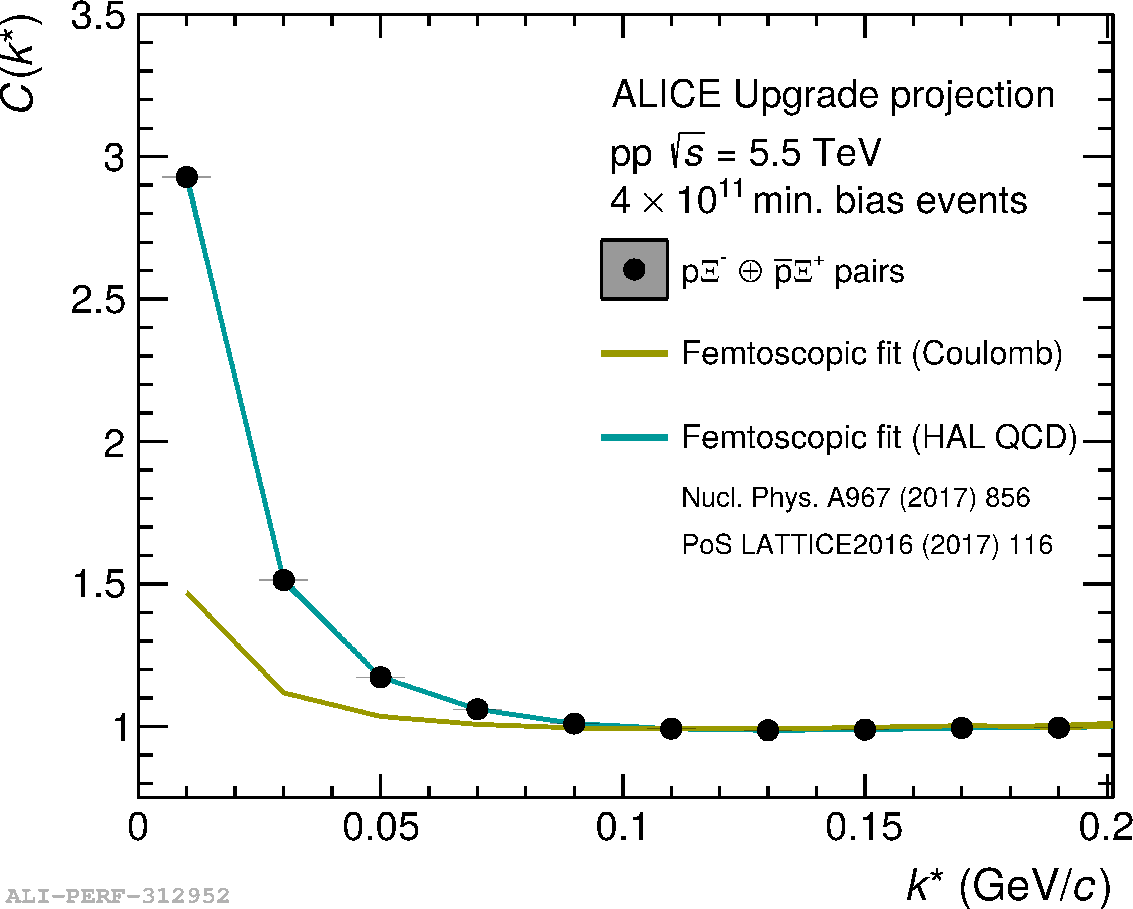
\includegraphics[width=.5\textwidth]{\main/lightflavour/figs/2018-11-15-2018-11-15-Projection_pXi_Model.pdf}
\caption{Expected p$\Xi^-$ correlation for pp collisions at $\sqrt{s} = 5.5$ TeV and $4\times 10^{11}$ minimum bias events, corresponding to $L_{int}~=~6~\mathrm{pb}^{-1}$.}
\label{pXiProj}
\end{figure}

Among the quantitative results obtained for the Run 2 samples, the first observation of the attractive p$\Xi^-$ interaction is worth being mentioned. 
Figure \ref{pXiProj} 
%\todo{Stefano P: as discussed last time, you should try to evaluate the errors taking into account also other models more than HAL QCD} 
shows the expected p$\Xi$ correlation for the Run 3 pp sample as a function of the relative momentum k*. 
The projection is obtained on the base of the current prediction by the HAL-QCD lQCD group that are in agreement with the Run 2 results.
The strong deviation from the Coulomb-only correlation function shows the effect of the strong attractive interaction 
and the expected statistics will allow for a quantitative determination of the scattering parameters and the test of different hadronic models.
The investigation will also be extended to the $\Sigma^0$ hyperon, since for the Run 3 and 4 samples we expect a total of 500.000 p$\Sigma^0$ pairs
to be used to study the femtoscopy correlation.

In summary, massive neutron stars with $M \sim 2M_{\bigodot}$ are very intriguing recent observations in relativistic astrophysics. 
An improved account of the two-body YN interaction, the three-body $\Lambda NN$ forces and the contribution of multi-strange hyperons in EoS is crucially important for more realistic description of the compact astrophysical objects, in particular, neutron and hybrid stars. The measurement of hyper-nuclei and hyperon correlations with the HL-LHC project are suggested as a promising tool for astrophysical applications.
